\documentclass{beamer}
\usetheme{CambridgeUS}
%%%%%%%%%%%%%%%%%%%%%%%%%%%%%%%%%%%%%%%%%%%%%%%%%%%%%%%
\setbeamercolor{block title}{bg=red!80!black, fg=white}
\setbeamercolor{block body}{bg=red!10, fg=black}
%%%%%%%%%%%%%%%%%%%%%%%%%%%%%%%%%%%%%%%%%%%%%%%%%%%%%%%
\usepackage[utf8]{vietnam}
\usepackage{tikz}

%%%%%%%%%%%%%%%%%%%%%%%%%%%%%%%%%%%%%%%%%%%%%%%%%%%%%%%
\AtBeginSection[]
{
\begin{frame}<beamer>
\frametitle{Nội dung}

\tableofcontents[
currentsection,
subsectionstyle=hide/hide,
subsubsectionstyle=hide/hide
]
\end{frame}
}
%%%%%%%%%%%%%%%%%%%%%%%%%%%%%%%%%%%%%%%%%%%%%%%%%%%%%%%
\title[{\makebox[.15\paperwidth]{MI4100 - Mật mã và độ phức tạp thuật toán}}]{Chủ đề: Mô phỏng tấn công hệ mật mã khóa công khai RSA bằng thuật toán LLL giảm lưới}
\author[Nhóm 8]{Nhóm 8}
\date[\today]{\today}
%%%%%%%%%%%%%%%%%%%%%%%%%%%%%%%%%%%%%%%%%%%%%%%%%%%%%%%
\begin{document}
%%%%%%%%%%%%%%%%%%%%%%%%%%%%%%%%%%%%%%%%%%%%%%%%%%%%%%%
% Trang tiêu đề cần có hình ảnh pictures/HUST2.jpeg
% Không chỉnh sửa gì
\begin{frame}
\begin{tikzpicture}[remember picture, overlay]
\node[anchor=center, inner sep=0pt] at (current page.center) {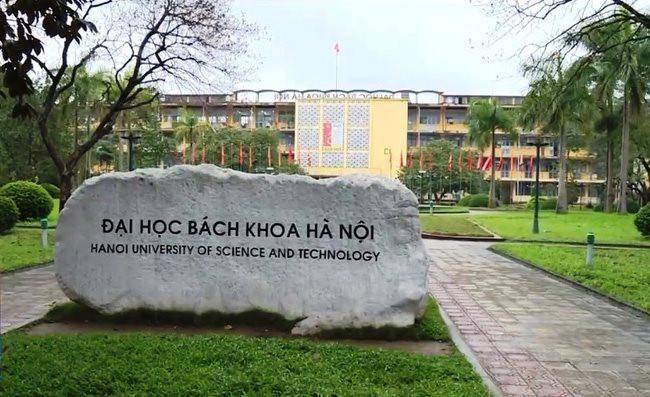
\includegraphics[width=\paperwidth, height=\paperheight]{pictures/HUST2.jpeg}};
\fill[white, opacity=0.8] (current page.south west) rectangle (current page.north east);
\end{tikzpicture}
\titlepage
\end{frame}
%%%%%%%%%%%%%%%%%%%%%%%%%%%%%%%%%%%%%%%%%%%%%%%%%%%%%%%
\begin{frame}{Danh sách thành viên}
\begin{block}{Nhóm 8}
\centering
\begin{tabular} {|l|c|}
\hline
Họ và tên & MSSV \\
\hline
Nguyễn Phan Anh & 20206113 \\
Nguyễn Việt Anh & 20206115 \\
Nguyễn Đình Anh & 20206111 \\
Nguyễn Thị Hoa & 20206199 \\
Vũ Văn Nghĩa & 20206205 \\
\hline
\end{tabular}
\end{block}
\end{frame}
%%%%%%%%%%%%%%%%%%%%%%%%%%%%%%%%%%%%%%%%%%%%%%%%%%%%%%%
\begin{frame}{Phân công thành viên}
\begin{block}{Phân công thành viên}
\begin{itemize}
\item Nguyễn Phan Anh: Lập kế hoạch, phân chia công việc, phân chia công việc, xxxxxxxxxxxxxxxxxxxxxxxxxxxxxx
\item Nguyễn Việt Anh: Lập kế hoạch, phân chia công việc, phân chia công việc, xxxxxxxxxxxxxxxxxxxxxxxxxxxxxx
\item Nguyễn Đình Anh: Lập kế hoạch, phân chia công việc, phân chia công việc, xxxxxxxxxxxxxxxxxxxxxxxxxxxxxx
\item Nguyễn Thị Hoa: Lập kế hoạch, phân chia công việc, phân chia công việc, xxxxxxxxxxxxxxxxxxxxxxxxxxxxxx
\item Vũ Văn Nghĩa: Lập kế hoạch, phân chia công việc, phân chia công việc, xxxxxxxxxxxxxxxxxxxxxxxxxxxxxx
\end{itemize}
\end{block}
\end{frame}
%%%%%%%%%%%%%%%%%%%%%%%%%%%%%%%%%%%%%%%%%%%%%%%%%%%%%%%
%! %%%%%%%%%%%%%%%%%%%%%%%%%%%%%%%%%%%%%%%%%%%%%%%%%%%%%%
%! %%%%%%%%%%%%%%%%%%%%%%%%%%%%%%%%%%%%%%%%%%%%%%%%%%%%%%
%! %%%%%%%%%%%%%%%%%%%%%%%%%%%%%%%%%%%%%%%%%%%%%%%%%%%%%%
%! %%%%%%%%%%%%%%%%%%%%%%%%%%%%%%%%%%%%%%%%%%%%%%%%%%%%%%
%! %%%%%%%%%%%%%%%%%%%%%%%%%%%%%%%%%%%%%%%%%%%%%%%%%%%%%%
\section{Tổng quan về hệ mật mã khóa công khai}
\subsection{Lịch sử}
\begin{frame}{Lịch sử}

\begin{itemize}
\item Hệ mật mã khóa công khai là một bước tiến lớn và là cuộc cách mạng trong lĩnh vực mật mã
\item Hệ mật mã khóa công khai được Diffie và Hellman đưa ra năm 1976
\end{itemize}

\begin{columns}

\begin{column}{0.4\textwidth}
\begin{figure}[H]
\centering
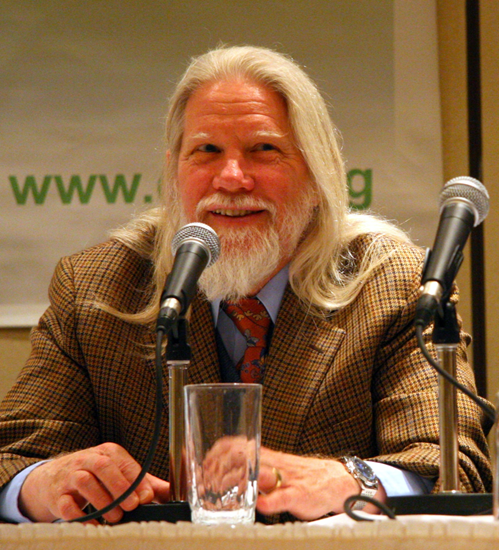
\includegraphics[scale = 0.4]{pictures/Bailey_Whitfield_Diffie.png}
\end{figure}
Bailey Whitfield 'Whit' Diffie\\ (sinh 05/06/1944 – 80 tuổi)
\end{column}

\begin{column}{0.4\textwidth}
\begin{figure}[H]
\centering
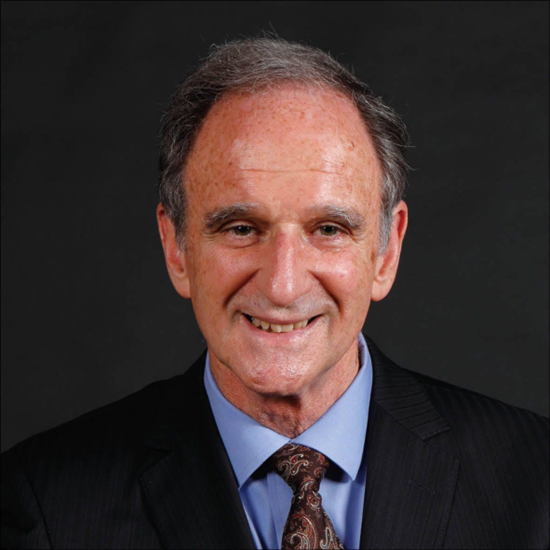
\includegraphics[scale = 0.4]{pictures/Martin_Edward_Hellman.png}
\end{figure}
Martin Edward Hellman\\(sinh 02/10/1945 - 79 tuổi)
\end{column}

\end{columns}
\end{frame}
%%%%%%%%%%%%%%%%%%%%%%%%%%%%%%%%%%%%%%%%%%%%%%%%%%%%%%%
\subsection{Khái niệm}
\begin{frame}{Khái niệm}

\begin{itemize}
\item Hệ mật mã khóa công khai là một dạng mật mã hoá cho phép người sử dụng trao đổi các thông tin mật mà không cần phải trao đổi các khoá chung bí mật trước đó
\item Việc mã hóa công khai được thực hiện bằng cách sử dụng một cặp khóa có quan hệ toán học với nhau là khóa công khai và khoá bí mật
\begin{itemize}
\item Khóa công khai: được công khai phổ biến - dùng để mã hóa
\item Khóa bí mật: được giữ bí mật - dùng để giải mã
\end{itemize}
\end{itemize}

$\Rightarrow$ Điều này đảm bảo hệ thống là không thể (hoặc rất khó) tìm ra khóa bí mật nếu chỉ biết khóa công khai

\end{frame}
%%%%%%%%%%%%%%%%%%%%%%%%%%%%%%%%%%%%%%%%%%%%%%%%%%%%%%%
\subsection{Mô hình tổng quát}
\begin{frame}{Mô hình tổng quát}
\begin{figure}[H]
\centering
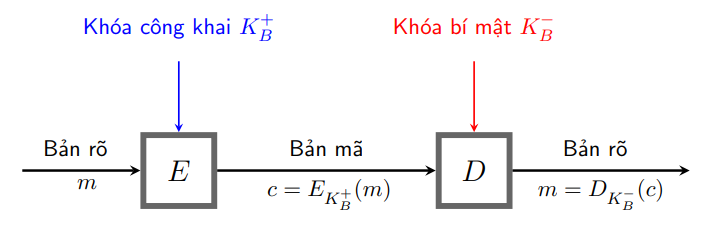
\includegraphics[scale = 0.6]{pictures/mo_hinh_tong_quat.png}
\end{figure}

\begin{block}{Nhận xét}
Hệ mật mã khóa công khai được gọi là hệ mật mã bất đối xứng vì mã hóa và giải mã sử dụng khóa khác nhau
\end{block}
\end{frame}
%%%%%%%%%%%%%%%%%%%%%%%%%%%%%%%%%%%%%%%%%%%%%%%%%%%%%%%
\subsection{Ưu, nhược điểm của hệ mã hóa công khai}
\begin{frame}{Ưu điểm}
\begin{itemize}
\item Thuật toán được viết một lần, công khai cho nhiều lần dùng, cho nhiều người dùng, họ chỉ cần giữ bí mật khóa riêng của mình
\item Khi biết các tham số ban đầu của hệ mã hóa, việc tính ra cặp khoá công khai và bí mật phải là "dễ", tức là trong thời gian đa thức
\item Khả năng lộ khóa bí mật khó hơn vì chỉ có một người giữ gìn. Nếu thám mã biết khoá công khai, cố gắng tìm khoá bí mật, thì chúng phải đương đầu với bài toán "khó"
\item Nếu thám mã biết khoá công khai và bản mã, thì việc tìm ra bản rõ cũng là bài toán "khó"
\end{itemize}
\end{frame}
%%%%%%%%%%%%%%%%%%%%%%%%%%%%%%%%%%%%%%%%%%%%%%%%%%%%%%%
\begin{frame}{Nhược điểm}
\begin{itemize}
\item Hệ mã hóa khóa công khai: mã hóa và giải mã chậm hơn hệ mã hóa khóa bí mật
\item Khả năng bị tấn công dạng tấn công người đứng giữa do kẻ tấn công lợi dụng việc phân phối khóa công khai để thay giả mạo gói tin
\end{itemize}
\end{frame}
%%%%%%%%%%%%%%%%%%%%%%%%%%%%%%%%%%%%%%%%%%%%%%%%%%%%%%%
\subsection{So sánh với mã đối xứng}
\begin{frame}{So sánh với mã đối xứng}

\end{frame}
%%%%%%%%%%%%%%%%%%%%%%%%%%%%%%%%%%%%%%%%%%%%%%%%%%%%%%%
%! %%%%%%%%%%%%%%%%%%%%%%%%%%%%%%%%%%%%%%%%%%%%%%%%%%%%%%
%! %%%%%%%%%%%%%%%%%%%%%%%%%%%%%%%%%%%%%%%%%%%%%%%%%%%%%%
%! %%%%%%%%%%%%%%%%%%%%%%%%%%%%%%%%%%%%%%%%%%%%%%%%%%%%%%
%! %%%%%%%%%%%%%%%%%%%%%%%%%%%%%%%%%%%%%%%%%%%%%%%%%%%%%%
%! %%%%%%%%%%%%%%%%%%%%%%%%%%%%%%%%%%%%%%%%%%%%%%%%%%%%%%

\end{document}

\subsection{Bảng chữ cái RSA}
\begin{frame}{Bảng chữ cái RSA}

\end{frame}
% \documentclass{beamer}
% \usepackage[utf8]{vietnam}
% \usepackage{amsmath}

% \begin{document}

% \begin{frame}{Thuật toán sinh khóa}

% \begin{enumerate}
% \item Chọn hai số nguyên tố đủ lớn, $p$ và $q$.
% \item Tính toán $n = pq$ và $\phi(n) = (p - 1)(q - 1)$.
% \item Chọn một số $e$ $(1 < e < \phi(n))$ sao cho $\text{gcd}(e, \phi(n)) = 1$.

% Giá trị $e$ sẽ được sử dụng trong mã hoá.
% \item Tìm một số $d$ sao cho $ed - 1$ chia hết cho $\phi(n)$, hay nói cách khác $d = e^{-1} \mod \phi(n)$. Giá trị $d$ sẽ được sử dụng để giải mã.
% \item Công khai khóa $K^+_B = (n, e)$ và giữ bí mật khóa $K^-_B = (n, d)$.
% \end{enumerate}

% \end{frame}

% \end{document}